\documentclass[10pt]{IEEEtran}
\usepackage[backend=biber,style=phys]{biblatex}
\usepackage{amsmath}
\usepackage{amsfonts}
\usepackage{amssymb}
\usepackage{caption}
\usepackage{graphicx}
\usepackage{hyperref}
\usepackage{hhline}
\usepackage{listings}
\usepackage{multirow}
\lstset{language=C++}
\usepackage{csquotes}
\usepackage{url} 
\graphicspath{{./images/}}
\addbibresource{alphaspectroscopy.bib}

\begin{document}

% Define document title and author
    \title{$\alpha$-Particle Spectroscopy with Si}
    \author{Jamison Lahman, Brandon Coleman, and Taylor Grueser
    \thanks{Instructor: Paul King}}
    \maketitle

% Write abstract here
\begin{abstract}
$^{226}$Ra is an unstable isotope with numerous, possible daughter
products.
Performing spectroscopy with a solid-state silicon detector, we are able to observe the alpha particles emitted during some of the decays. Most transitions have relatively small half-lives compared to the decay of  $^{226}$Ra and $^{210}$Pb. Their constituent half-lives are approximately 1600 years and 22.20 years respectively. Comparing these two decay rates we are able to estimate the age of the sample of $^{226}$Ra. We found the age of our sample to be 12.17$\pm$0.20 years while the accepted value is approximately 10.47 years. In addition, by comparing the cross-sectional area to the number of counts we were able to estimate an activity of 1.799$\pm$0.006 kBq while the accepted activity was approximately 3.235 kBq.
\end{abstract}

\section{Introduction \& Theory}

By measuring the decay rates of of the daughter products of $^{226}$Ra, it is possible to estimate the age since the Radon was in its pure state.\cite{blackboard} With the exception of $^{226}$Ra and $^{210}$Pb, the half-lives (t$_{1/2}$), the time required for half a sample to have decayed, are all less than a week. The half-lives of $^{226}$Ra and $^{210}$Pb are 1600$\pm$7 years and 22.20$\pm$0.22 years respectively.\cite{sonzogni} Given this decay time disparity, after about a few weeks of the $^{226}$Ra decaying, there are a sufficient number of daughter particles that they decay at a rate of the daughter decay is virtually equivalent to the previous decay rate, with the exception of the $^{210}$Pb. With the $^{210}$Pb's half-life being about 22 years, we are effectively able to estimate what the decay rate of $^{226}$Ra was 22 years ago. The relationship of these two rates can be therefore be used to estimate the age. Because the $^{210}$Pb decays through beta decay, we are only able to measure the $^{210}$Po decay rate but they are effectively the same given previous arguments. The most prominent alpha decays are given by Tab \ref{tab:decays} while the entire decay chain is shown in Fig. \ref{fig:chain}.
    \begin{table}[!h]
        % Center the table
        \begin{center}
        % Title of the table
        \caption{Alpha Decays of $^{226}$Ra and Daughter Products}
        \label{tab:decays}
        % Table itself: here we have two columns which are centered and have lines to the left, right and in the middle: |c|c|
        \begin{tabular}{|c|c|c|c|}
            % To create a horizontal line, type \hline
            \hline
            Element & Alpha Energy (keV) & Uncertainty (keV) & Likelihood \\
            \hline
            $^{226}$Ra & 4784.34 & 0.25 & 93.84\% \\
            \hline
            $^{210}$Po & 5304.33 & 0.70 & 100\% \\ 
            \hline         
            $^{222}$Rn & 5489.48 & 0.30 & 100\% \\
            \hline
            $^{218}$Po & 6002.35 & 0.90 & 99.98\% \\
            \hline
            $^{214}$Po & 7686.82 & 0.70 & 100\% \\
            \hline
        \end{tabular}
        \end{center}
        The energy and likelihood the elements following Fig. \ref{fig:chain} decaying through alpha emission. The remaining alpha decay paths have likelihoods of $\textless$ 1\%\cite{sonzogni}. Likewise, the beta decays are un-observable given our detector\cite{blackboard}.
    \end{table}

    \begin{figure}[!h]
        % Center the figure.
        \begin{center}
        % Include the eps file, scale it such that it's width equals the column width. You can also put width=8cm for example...
        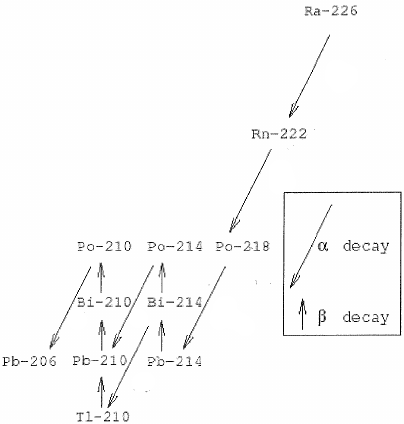
\includegraphics[width=\columnwidth]{chain.png}
        % Create a subtitle for the figure.
       \caption{The possible decay paths for the initial $^{226}$Ra sample. Alpha decays are down pointing arrows while beta decays point upwards. Corresponding energies and decay likelihoods are given in Tab. \ref{tab:decays}\cite{blackboard}.}
        % Define the label of the figure. It's good to use 'fig:title', so you know that the label belongs to a figure.
        \label{fig:chain}
        \end{center}
    \end{figure}
    
The rate at which a sample decays is\cite{blackboard},
	\begin{equation}
		N = N_0 \exp(-t/\tau),
	\end{equation}
where $N$ is the number of atoms remaining, $N_0$ is the initial number of atoms, $t$ is the time since the sample was in its pure form, and $\tau$ is the mean lifetime. The mean lifetime is defined as,
	\begin{equation}
		\tau \equiv \frac{t_{1/2}}{\ln(2)}.
	\end{equation}

The activity, $A$, of the sample is defined as the rate at which the atoms decay, therefore it is the time derivative of Eq. (1)\cite{blackboard};
	\begin{equation}
		A \equiv -\frac{d N}{dt} = \frac{N}{\tau} = \frac{N_0 \exp(-t/\tau)}{\tau} = A_0\exp(-t/\tau).
	\end{equation}
Where $A_0$ is the activity at $t=0$.

We can combine Eqs. (1) and (3) to find the decay rate of a daughter product denoted as $N_D$\cite{blackboard},
	\begin{equation}
		\frac{d N_D}{dt} = \frac{d N}{dt} + \frac{N_D}{\tau_D} = \frac{N_D}{\tau_D} - \frac{N_0 \exp(-t/\tau)}{\tau}.
	\end{equation}
For products that decay relatively quickly, the $N_D$ term effectively goes to zero and it is easy to see that the input decay rate is roughly equivalent to the output decay rate.

Setting $N_{D} = 0$ for $t = 0$, the differential from Eq. (4) can be solved producing,
	\begin{equation}
		\frac{N_D}{\tau_D} = \frac{N_0}{\tau - \tau_D}[\exp(-t/\tau)-\exp(-t/\tau_D)].
	\end{equation}

Combining Eqs. (3) and (5), we can define the ratio of the two decay rates, $R$, which is given by,
	\begin{equation}
		R \equiv \frac{N_D\ \tau}{N\ \tau_D} = \frac{\tau}{\tau-\tau_D}[1-\exp(-t/\tau_D+t/\tau)].
	\end{equation}
Solving Eq. (6) for $t$ yields\cite{blackboard},
	\begin{equation}
		t = -\frac{\tau\ \tau_D}{\tau-\tau_D}\ln\left(1-R\frac{\tau-	\tau_D}{\tau}\right).
	\end{equation}

\section{Experimental Details}


The $^{226}$Ra is placed inside a vacuum chamber. The detector, BA-024-300-500 by ORTEC Incorporated, is connected to a pre-amp by a single, coaxial cable. The pre-amp is given a voltage bias of 250 volts. The pre-amp output is then sent to an amplifier where it then sent to an ADC. The ADC data is then stored on a computer. The pre-amp and amplifier are both set to amplify by 10x in each.

The detector has an active area of 3cm$^{2}$, an alpha resolution of 20.3 keV, and a noise width of 16.0 keV. 

In order to determine the activity of the sample, we must find the ratio of the detector's area on a sphere with a radius that is the furthest distance to the detector. The sample is approximately $8.80\pm0.05$cm from the detector. Using geometry, we can find the radius of the detector, r,
	\begin{equation}
		a = \pi r^2 \Rightarrow r = \sqrt{\frac{a}{\pi}}=\sqrt{\frac{3\text{cm}^2}{\pi}} = 0.98\text{cm}.
	\end{equation}
The radius of the sphere, c, is found using the Pythagorean Theorem:
	\begin{equation}
		c = \sqrt{r^2+s^2} = \sqrt{(0.98\text{cm})^2+(8.80\text{cm})^2} = 8.85\text{cm}.
	\end{equation}
Where $s$ is the length separating the detector and sample. The total area of the sphere is then
	\begin{equation}
		SA = 4\pi c^2 = 4\pi (8.85\text{cm})^2 = 1201\text{cm}^2.
	\end{equation}
The error is therefore,
	\begin{equation}
		\sigma_{SA} = \sigma_s \frac{\partial SA}{\partial s}= (0.05\text{cm})(8\pi8.85\text{cm}) = 12.29\text{cm}^2.
	\end{equation}

The angle, $\theta$, separating the azimuth from the point which the detector intersects the sphere is simply,
	\begin{equation}
		\theta = \tan^{-1}(r/s) = \tan^{-1}\left(\frac{0.98\text{cm}}{8.80\text{cm}}\right) = 0.1106.
	\end{equation}
The total area on the sphere by the detector is therefore
	\begin{eqnarray}
		\begin{array}{rl}
			{SA}_r&=\iint r^2\sin(\theta)d\phi d\theta \\
			&=(8.85\text{cm})^2\int_0^{2\pi}\int_0^{0.1106}\sin(\theta)d\phi d\theta = 3.01\text{cm}^2.
		\end{array}
	\end{eqnarray}

The ratio of the two areas is then
	\begin{equation}
		\frac{{SA}_r}{SA} = \frac{3.01\text{cm}^2}{1201\text{cm}^2} = 0.2505\%.
	\end{equation}
While the error is given by,
	\begin{equation}
		\sigma_{\%} = \frac{SA_r}{SA} \sqrt{ \left(\frac{\sigma_{SA_{r}}}{SA_r}\right)^2+\left( \frac{\sigma_{SA}}{SA}\right)^2} = 0.0026\%.
	\end{equation}
This indicates that our detector is going to receive about a quarter of a percent of the total alpha-particle emitted by the sample. We can use this fact to find the total number of alphas emitted over a given interval, thus the activity of the sample.

The $^{226}$Ra sample had an initial activity of 3.266 kBq and was approximately 3820 days old. Using Eq. (3), the accepted activity at the time of data acquisition should be approximately 3.235 kBq.

We took data over the course of four days, with times ranging from 6 to 40 minutes for a total of 4 head-on sets. We also took one set of data with vanadium foil in between the sample and the detector.
\section{Data}

As expected, we were able to detect the five alpha emissions detailed in Tab. \ref{tab:decays}. In addition, the size of the $^{210}$Po was much smaller than the other peaks which were relatively the same size. An example output histogram is shown in Fig. \ref{fig:hist}.
    \begin{figure}[!h]
        % Center the figure.
        \begin{center}
        Alpha Decays of $^{226}$Ra and Daughter Products
        % Include the eps file, scale it such that it's width equals the column width. You can also put width=8cm for example...
        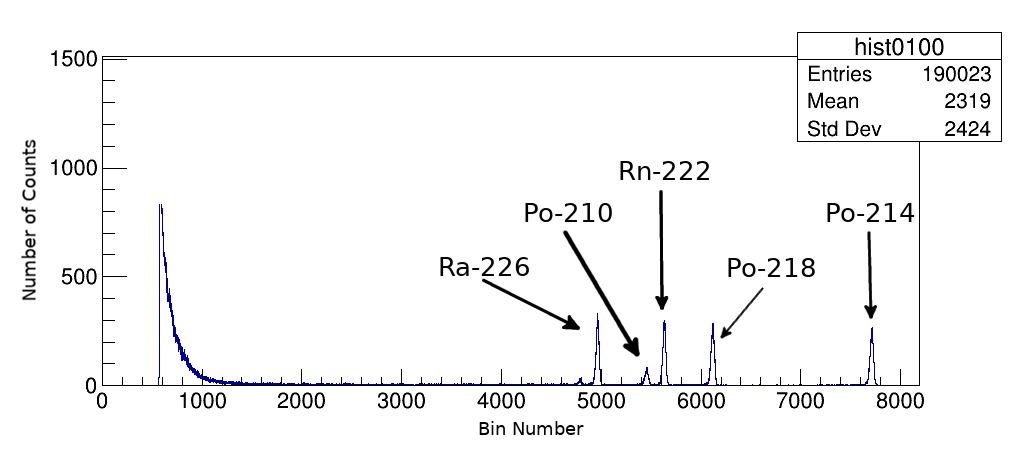
\includegraphics[width=\columnwidth]{hist0100.png}
        % Create a subtitle for the figure.
       \caption{An example histogram with the most prominent peaks labeled. The four largest peaks are all similar in size while the Po-210 is substantially smaller.}
        % Define the label of the figure. It's good to use 'fig:title', so you know that the label belongs to a figure.
        \label{fig:hist}
        \end{center}
    \end{figure}
    
    \begin{table}[!h]
        % Center the table
        \begin{center}
        % Title of the table
        \caption{Observed 4784 keV Alpha Decay of $^{226}$Ra}
        \label{tab:ra226}
        % Table itself: here we have two columns which are centered and have lines to the left, right and in the middle: |c|c|
        \begin{tabular}{|c|c|c|c|c|c|}
            % To create a horizontal line, type \hline
            \hline
            Date & Time (s) & \# of Counts & Mean Bin & RMS & $\sigma_{\bar{x}}$ \\
            \hline
            2/13/17 & 360 & 1486 & 4958 & 17.97 & 0 \\
            \hline
            2/15/17 & 2500 & 10735 & 4963 & 15.25 & 0 \\
            \hline
            2/19/17 & 900 & 4270 & 4953 & 17.62 & 0 \\
            \hline
            2/22/17 & 900 & 3595 & 4960 & 17.11 & 0 \\
            \hline
        \end{tabular}
        \end{center}
        The time, number of counts, and peak characteristics for peaks associated to the alpha decay of $^{226}$Ra, specifically the 4784.34 keV alpha particle. Runs were taken over four, separate days.
    \end{table}    
    
    \begin{table}[!h]
        % Center the table
        \begin{center}
        % Title of the table
        \caption{Observed Alpha Decays of $^{210}$Po}
        \label{tab:po210}
        % Table itself: here we have two columns which are centered and have lines to the left, right and in the middle: |c|c|
        \begin{tabular}{|c|c|c|c|c|c|}
            % To create a horizontal line, type \hline
            \hline
            Date & Time (s) & \# of Counts & Mean Bin & RMS & $\sigma_{\bar{x}}$ \\
            \hline
            2/13/17 & 360 & 565 & 5450 & 34.68 & 1 \\
            \hline
            2/15/17 & 2500 & 3589 & 5451 & 31.13 & 1 \\
            \hline
            2/19/17 & 900 & 1329 & 5445 & 29.33 & 1 \\
            \hline
            2/22/17 & 900 & 1339 & 5448 & 34.33 & 1 \\
            \hline
        \end{tabular}
        \end{center}
        The time, number of counts, and peak characteristics for 4 peaks associated to the alpha decay of $^{210}$Po.
    \end{table}
    
    \begin{table}[!h]
        % Center the table
        \begin{center}
        % Title of the table
        \caption{Observed Alpha Decays of $^{222}$Rn}
        \label{tab:rn222}
        % Table itself: here we have two columns which are centered and have lines to the left, right and in the middle: |c|c|
        \begin{tabular}{|c|c|c|c|c|c|}
            % To create a horizontal line, type \hline
            \hline
            Date & Time (s) & \# of Counts & Mean Bin & RMS & $\sigma_{\bar{x}}$ \\
            \hline
            2/13/17 & 360 & 1668 & 5625 & 21.25 & 1 \\
            \hline
            2/15/17 & 2500 & 11267 & 5630 & 18.13 & 0 \\
            \hline
            2/19/17 & 900 & 4057 & 5620 & 19.10 & 0 \\
            \hline
            2/22/17 & 900 & 3989 & 5626 & 20.44 & 0 \\
            \hline
        \end{tabular}
        \end{center}
        The time, number of counts, and peak characteristics for 4 peaks associated to the alpha decay of $^{222}$Rn.
    \end{table}
    
    \begin{table}[!h]
        % Center the table
        \begin{center}
        % Title of the table
        \caption{Observed Alpha Decays of $^{218}$Po}
        \label{tab:po218}
        % Table itself: here we have two columns which are centered and have lines to the left, right and in the middle: |c|c|
        \begin{tabular}{|c|c|c|c|c|c|}
            % To create a horizontal line, type \hline
            \hline
            Date & Time (s) & \# of Counts & Mean Bin & RMS & $\sigma_{\bar{x}}$ \\
            \hline
            2/13/17 & 360 & 1673 & 6111 & 20.03 & 0 \\
            \hline
            2/15/17 & 2500 & 11614 & 6115 & 18.29 & 0 \\
            \hline
            2/19/17 & 900 & 4270 & 6104 & 18.08 & 0 \\
            \hline
            2/22/17 & 900 & 4084 & 6112 & 19.78 & 0 \\
            \hline
        \end{tabular}
        \end{center}
        The time, number of counts, and peak characteristics for 4 peaks associated to the alpha decay of $^{218}$Po.
    \end{table}
    
     \begin{table}[!h]
        % Center the table
        \begin{center}
        % Title of the table
        \caption{Observed Alpha Decays of $^{214}$Po}
        \label{tab:po214}
        % Table itself: here we have two columns which are centered and have lines to the left, right and in the middle: |c|c|
        \begin{tabular}{|c|c|c|c|c|c|}
            % To create a horizontal line, type \hline
            \hline
            Date & Time (s) & \# of Counts & Mean Bin & RMS & $\sigma_{\bar{x}}$ \\
            \hline
            2/13/17 & 360 & 1508 & 7703 & 19.25 & 1 \\
            \hline
            2/15/17 & 2500 & 10515 & 7708 & 18.27 & 0 \\
            \hline
            2/19/17 & 900 & 3867 & 7695 & 18.36 & 0 \\
            \hline
            2/22/17 & 900 & 3643 & 7703 & 19.29 & 0 \\
            \hline
        \end{tabular}
        \end{center}
        The time, number of counts, and peak characteristics for 4 peaks associated to the alpha decay of $^{214}$Po.
    \end{table}
    
\newpage    
    
\section{Results}

Plotting the literature energy from Tab. \ref{tab:decays} as the dependent variable and using the mean bins from Tabs. \ref{tab:ra226}, \ref{tab:po210}, \ref{tab:rn222}, \ref{tab:po218}, and \ref{tab:po214} as the independent variable, we used a least squares linear regression\cite{bevington},
\begin{eqnarray}
a &=& \frac{1}{\Delta}\left(\sum\frac{1}{\sigma_i^2}\sum\frac{x_i y_i}{\sigma_i^2}-\sum \frac{x_i}{\sigma_i^2}\sum\frac{y_i}{\sigma_i^2}\right) \\
b &=& \frac{1}{\Delta}\left(\sum\frac{x_i^2}{\sigma_i^2}\sum\frac{y_i}{\sigma_i^2}-\sum\frac{x_i}{\sigma_i^2}\sum\frac{x_i y_i}{\sigma_i^2}\right) \\
\Delta &=& \sum\frac{1}{\sigma_i^2}\sum\frac{x_i^2}{\sigma_i^2}-\left(\sum\frac{x_i}{\sigma_i^2}\right)^2.
\end{eqnarray}
Additionally, the errors of the fit are given by\cite{bevington},
\begin{eqnarray}
\sigma_a^2 &=& \frac{1}{\Delta}\sum\frac{1}{\sigma_i^2} \\
\sigma_b^2 &=& \frac{1}{\Delta}\sum\frac{x_i^2}{\sigma_i^2} \\
\text{cov}(a,b) &=& \frac{-1}{\Delta}\sum\frac{x_i}{\sigma_i^2}.
\end{eqnarray}
the following energy calibrations were established for February 13th, 15th, 19th and 22nd respectively:
\begin{eqnarray}\begin{array}{c}
E_{13} = 1.06\text{E-}3\pm 3.72\text{E-}7(\bar{x})-0.458\pm 2.16\text{E-}3, \\
\text{cov}(a,b) = -7.94\text{E-}10, \\
E_{15} = 1.06\text{E-}3\pm 2.75\text{E-}7(\bar{x})-0.463\pm 1.52\text{E-}3, \\
\text{cov}(a,b) = -4.16\text{E-}10, \\
E_{19} = 1.06\text{E-}3\pm 2.70\text{E-}7(\bar{x})-0.462\pm 1.48\text{E-}3, \\
\text{cov}(a,b) = -3.95\text{E-}10, \\
E_{22} = 1.06\text{E-}3\pm 2.42\text{E-}7(\bar{x})-0.471\pm 1.42\text{E-}3, \\
\text{cov}(a,b) = -3.81\text{E-}10,
\end{array}
\end{eqnarray}
where $E$ is the corresponding energy (in MeV), and $\bar{x}$ is the mean bin of the peak.
    \begin{figure}[!h]
        % Center the figure.
        \begin{center}
        % Include the eps file, scale it such that it's width equals the column width. You can also put width=8cm for example...
        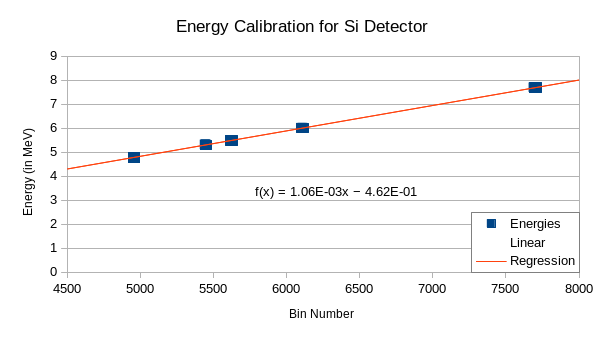
\includegraphics[width=\columnwidth]{energy.png}
        % Create a subtitle for the figure.
       \caption{The energy calibration for the Si detector using a weighted average defined by Bevington (2003) alongside using Eqs. (16), (17), and (18).}
        % Define the label of the figure. It's good to use 'fig:title', so you know that the label belongs to a figure.
        \label{fig:energy}
        \end{center}
    \end{figure}
    
    \begin{figure}[!h]
        % Center the figure.
        \begin{center}
        % Include the eps file, scale it such that it's width equals the column width. You can also put width=8cm for example...
        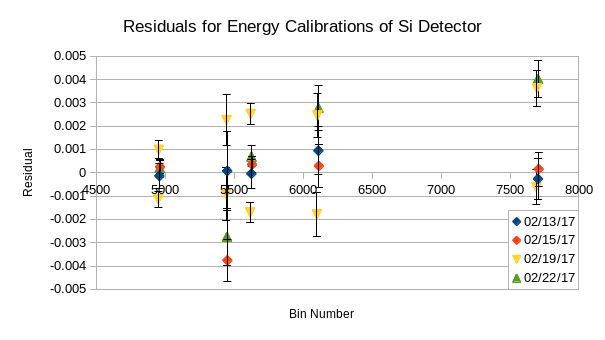
\includegraphics[width=\columnwidth]{energyresidual.png}
        % Create a subtitle for the figure.
       \caption{Residuals from energy calibrations found using Eqs. (16), (17), and (18). The calibrations were determined separately with respect solely to the date the data was acquired.}
        % Define the label of the figure. It's good to use 'fig:title', so you know that the label belongs to a figure.
        \label{fig:energyres}
        \end{center}
    \end{figure}


Dividing the number of counts by the times from Tabs. \ref{tab:ra226}, \ref{tab:po210}, \ref{tab:rn222}, \ref{tab:po218}, and \ref{tab:po214}, by the likelihoods of alpha decay from Tab. \ref{tab:decays} and by the ratio of the detector area to the total area of the encapsulating sphere from Eq. (13), we find the total number of counts per unit time. 

Using a weighted average defined in Bevington (2003), we were able to estimate the activity of the sample to be,
	\begin{equation}
		\textless A\textgreater = 1.799\pm0.006\text{ kBq}.
	\end{equation}
	
Analyzing the error propagation, we found the that about 80\% of the error was from the error in the area of the sphere while the remaining 20\% is from the uncertainty in the number of counts.

Dividing the number of counts from Tabs. \ref{tab:ra226}, \ref{tab:po210}, \ref{tab:rn222}, \ref{tab:po218}, and \ref{tab:po214} by the likelihoods of alpha decay from Tab. \ref{tab:decays}, we can then use Eq. (6) to find the decay ratio of the sample for each set. The results are shown in Tab. \ref{tab:R}.

     \begin{table}[!h]
        % Center the table
        \begin{center}
        % Title of the table
        \caption{Ratio of Alpha Particles from $^{210}$Po to $^{226}$Ra}
        \label{tab:R}
        % Table itself: here we have two columns which are centered and have lines to the left, right and in the middle: |c|c|
        \begin{tabular}{|c|c|c|c|c|c|c|}
            % To create a horizontal line, type \hline
            \hline
            Date & N; $^{226}$Ra & RMS & N; $^{210}$Po & RMS & $R$ & $\sigma_R$ \\
            \hline
            2/13/17 & 1584 & 19.15 & 565 & 34.68 & 0.357 & 0.022 \\
            \hline
            2/15/17 & 11439 & 16.25 & 3589 & 31.68 & 0.3138 & 0.0275\\
            \hline
            2/19/17 & 4550 & 18.78 & 1329 & 29.33 & 0.2921 & 0.0065 \\
            \hline
            2/22/17 & 3831 & 18.23 & 1339 & 34.33 & 0.3495 & 0.0091 \\
            \hline
        \end{tabular}
        \end{center}
The number of counts, adjusted for the specific alpha decay likelihood, from the $^{210}$Po and $^{226}$Ra decays. $R$ is the ratio of the number of counts of each peak. 
    \end{table}
Using a weighted average defined in Bevington (2003), we were able to estimate the average decay ratio:
	\begin{equation}
		\textless R\textgreater = 0.3170\pm0.022.
	\end{equation}

Inserting the ratios from Tab. \ref{tab:R} into Eq. (7) with accepted values of mean lifetimes from NuDat\cite{sonzogni}, we calculated approximate ages of the sample as shown in Tab. \ref{tab:t}

     \begin{table}[!h]
        % Center the table
        \begin{center}
        % Title of the table
        \caption{Age from the Decay Ratio of $^{210}$Po and $^{226}$Ra}
        \label{tab:t}
        % Table itself: here we have two columns which are centered and have lines to the left, right and in the middle: |c|c|
        \begin{tabular}{|c|c|c|c|c|}
            % To create a horizontal line, type \hline
            \hline
            Date & $R$ & $\sigma_R$ & $t$ (yrs) & $\sigma_t$\\
            \hline
            2/13/17 & 0.357 & 0.022 & 14.1 & 1.0\\
            \hline
            2/15/17 & 0.3138 & 0.0275 & 12.02 & 0.21 \\
            \hline
            2/19/17 & 0.2921 & 0.0065 & 11.03 & 0.35\\
            \hline
            2/22/17 & 0.3495 & 0.0091 & 13.73 & 0.45\\
            \hline
        \end{tabular}
        \end{center}
The decay ratio, $R$, of the $^{210}$Po and $^{226}$Ra decays. Using Eq. (7), we were able to estimate the age of the sample, $t$.
    \end{table}
Again using a weighted average, we find the average age of the sample to be,
	\begin{equation}
		\textless t\textgreater = 12.17\pm0.20\text{ years}.
	\end{equation}
	
Performing an analysis on the error propagation, we find that approximately 75\% of the error is from the uncertainty of the mean lifetime of the $^{210}$Pb while the remaining 25\% is from the uncertainty in the decay ratio.

Only one run, taken on February 19th, was ran with a substance in between the detector and source. Comparing Fig. \ref{fig:1001_4958} which had vanadium foil with Fig. \ref{fig:0000_4958} which had no material, one can see three major events happened to the peak. First, the peak was shifted about 500 bins to the left. Using the energy calibration for February 19th from Eq. (22), we find that the bin shift correlates to an energy shift of roughly $543$ keV. The energy loss was roughly 10\% of the total energy of the un-obstructed alpha particle. Second, the shape of the peak changed as the peak became skewed left. Lastly, the distribution drastically changed. The RMS increased by nearly 4 times.

    \begin{figure}[!h]
        % Center the figure.
        \begin{center}
        $^{226}$Ra Peak With Vanadium Foil
        % Include the eps file, scale it such that it's width equals the column width. You can also put width=8cm for example...
        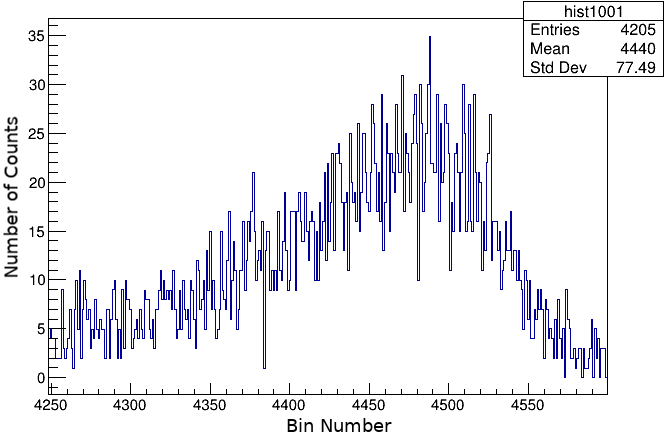
\includegraphics[width=\columnwidth]{1001_4958.png}
        % Create a subtitle for the figure.
       \caption{The $^{226}$Ra peak with vanadium foil in between the detector and sample. Notice the bin position and distribution of counts.}
        % Define the label of the figure. It's good to use 'fig:title', so you know that the label belongs to a figure.
        \label{fig:1001_4958}
        \end{center}
    \end{figure}
    
    \begin{figure}[!h]
        % Center the figure.
        \begin{center}
        $^{226}$Ra Peak With No Foil
        % Include the eps file, scale it such that it's width equals the column width. You can also put width=8cm for example...
        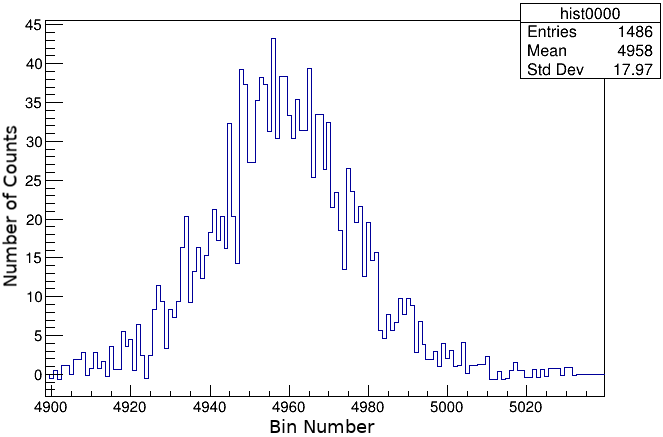
\includegraphics[width=\columnwidth]{0000_4958.png}
        % Create a subtitle for the figure.
       \caption{The $^{226}$Ra peak with no foil in between the detector and sample. Notice the bin position and distribution of counts.}
        % Define the label of the figure. It's good to use 'fig:title', so you know that the label belongs to a figure.
        \label{fig:0000_4958}
        \end{center}
    \end{figure}

\section{Conclusion}

Performing spectroscopy with a solid-state silicon detector, we were able to observe the alpha particles emitted during some of the decays. We showed it was possible to approximately estimate the age of a sample by comparing the two decay rates of $^{226}$Ra and $^{210}$Po. We found the age of our sample to be 12.17$\pm$0.20 years while the accepted value is approximately 10.47 years. In addition, by comparing the cross-sectional area to the number of counts we were able to estimate an activity of 1.799$\pm$0.006 kBq while the accepted activity was approximately 3.235 kBq. Neither values are withing a few standard errors, however the detector we used was malfunctioning and ended up needing replaced, likely introducing systematic errors.

\section{acknowledgments}
I would like to thank my lab partners, Brandon Coleman and Taylor Grueser, who helped with the setup, data acquisition and analysis for this report.
\printbibliography

\end{document}

% This is how you include a eps figure in your document. LaTeX only accepts EPS or TIFF files.
%    \begin{figure}[!hbt]
        % Center the figure.
%        \begin{center}
        % Include the eps file, scale it such that it's width equals the column width. You can also put width=8cm for example...
%        \includegraphics[width=\columnwidth]{}
        % Create a subtitle for the figure.
%       \caption{Simulation results on the AWGN channel. Average throughput $k/n$ vs $E_s/N_0$.}
        % Define the label of the figure. It's good to use 'fig:title', so you know that the label belongs to a figure.
%        \label{fig:tf_plot}
%        \end{center}
%    \end{figure}

    % This is how you define a table: the [!hbt] means that LaTeX is forced (by the !) to place the table exactly here (by h), or if that doesnt work because of a pagebreak or so, it tries to place the table to the bottom of the page (by b) or the top (by t).
%    \begin{table}[!hbt]
        % Center the table
%        \begin{center}
        % Title of the table
%        \caption{Simulation Parameters}
%        \label{tab:simParameters}
        % Table itself: here we have two columns which are centered and have lines to the left, right and in the middle: |c|c|
%        \begin{tabular}{|c|c|}
            % To create a horizontal line, type \hline
%            \hline
            % To end a column type &
            % For a linebreak type \\
%            Information message length & $k=16000$ bit \\
%            \hline
%            Radio segment size & $b=160$ bit \\
%            \hline
%            Rate of component codes & $R_{cc}=1/3$\\
%            \hline
%            Polynomial of component encoders & $[1 , 33/37 , 25/37]_8$\\
%            \hline
%        \end{tabular}
%        \end{center}
%    \end{table}

% You can cite a book or paper by using \cite{reference}.

% You can reference tables and figure by using the \ref{label} command. Each table and figure needs to have a UNIQUE label.
%Figures and tables should be labeled and numbered, such as in Table~\ref{tab:simParameters} and Fig.~\ref{fig:tf_plot}.
